\documentclass[12pt]{article}

\usepackage{graphicx}
\usepackage{float}
\usepackage{array}
\usepackage{amsmath}
\usepackage{amsfonts}
\usepackage{amsthm}
\usepackage{enumitem}
\usepackage{subcaption}
\usepackage[font={small,it}]{caption}
\graphicspath{{./images/}}



\makeatletter
\setlength{\@fptop}{0pt}
\makeatother


\title{Segmentation via Clustering}
\author{Hanwen Zhao}
\date{}

\begin{document}
\maketitle

\begin{abstract}
In this report we will use clustering algorithms to segment images and use these segmentation to identify foreground and background objects. Eventually, we will transfer foreground objects from one image to another.
\end{abstract}

\section{Clustering Algorithms}
Clustering is a machine learning technique which separate data points into groups. With a given data set, we can classify them into specific groups as we demand. In this section, we will discuss two popular clustering algorithms. The approach we used is from bottom up, pixels belong together because they look similar. In this section, we will discuss two different popular clustering algorithms: K-Means Clustering and Hierarchical Agglomerative Clustering.

\subsection{K-Means Clustering}
The idea behind the K-Means Clustering Algorithm is very simple: 

\begin{itemize}
	\item we randomly initialize the k cluster centers
	\item for each point p, find and assign to closest cluster $c_i$
  	\item set $c_i$ to be the mean of the points in cluster i, this is the new center
  	\item repeat steps until $c_i$ remain the same
\end{itemize}
\noindent
The following figure shows the iteration steps of K-Means Clustering Algorithm.


\begin{figure}[t!]
    \centering
    \begin{subfigure}[b]{0.25\textwidth}
        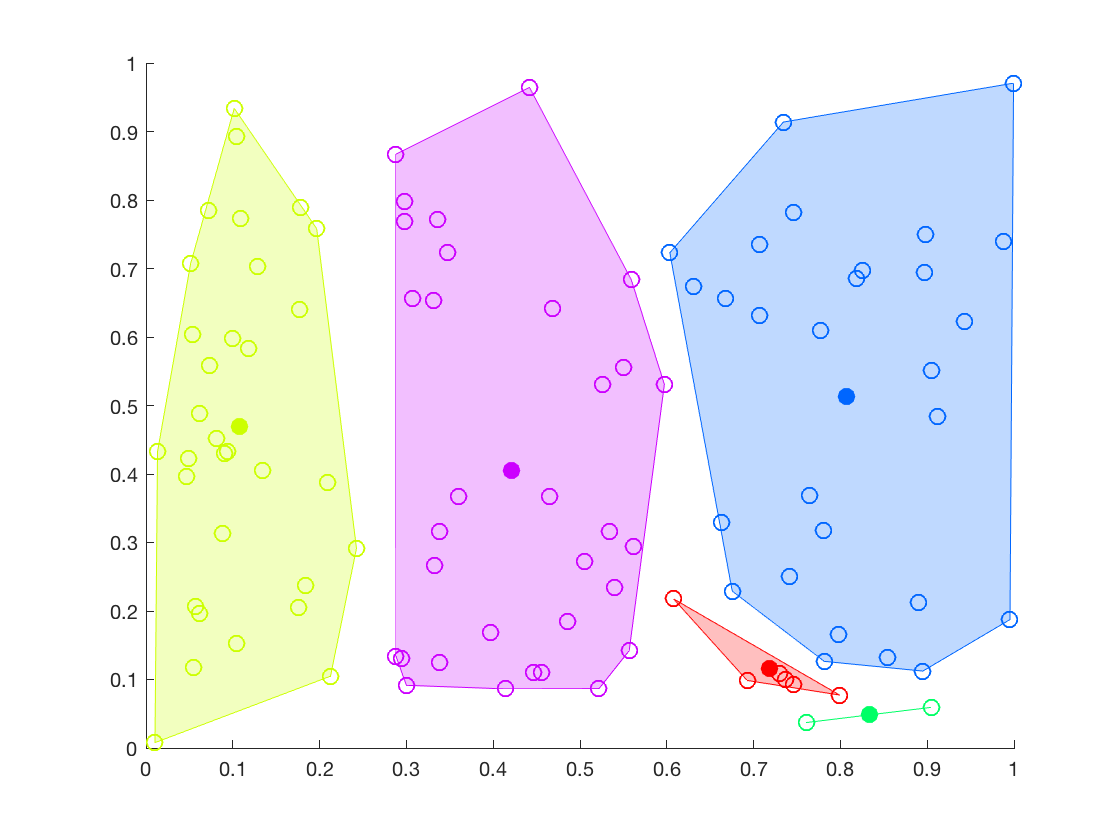
\includegraphics[width=\textwidth]{k-means_1}
    \end{subfigure}
    \begin{subfigure}[b]{0.25\textwidth}
        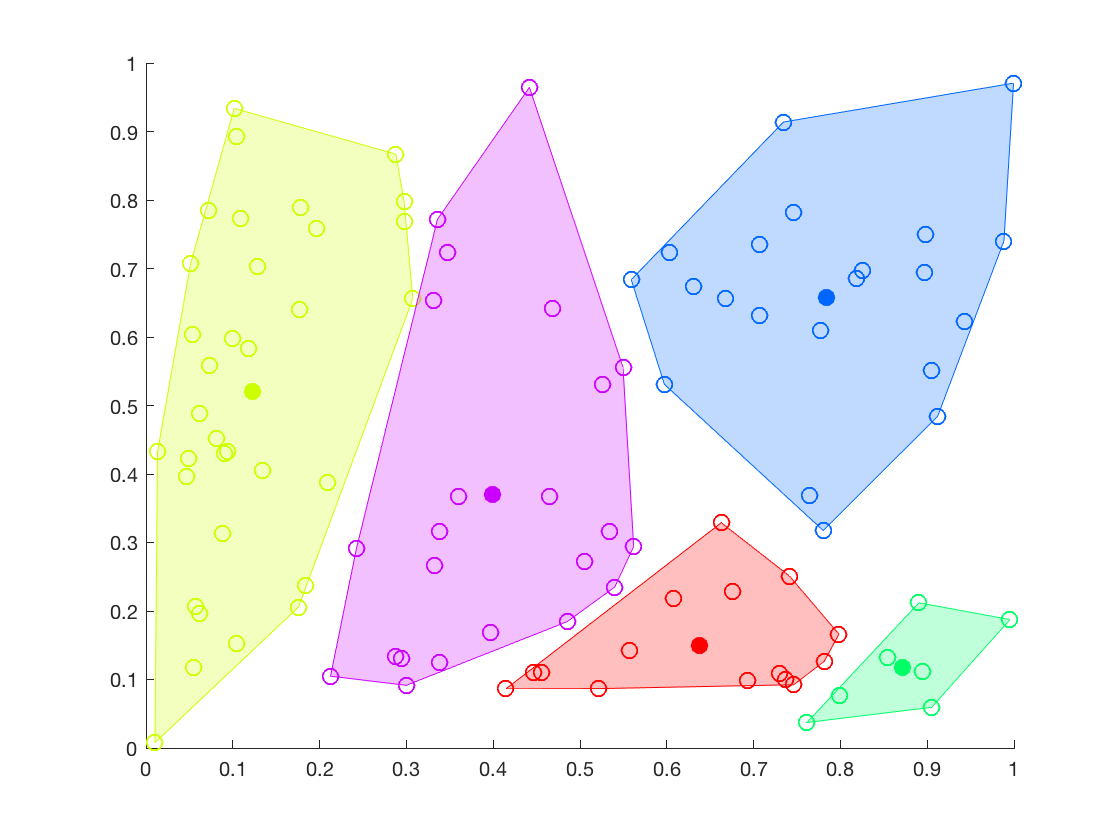
\includegraphics[width=\textwidth]{k-means_2}
    \end{subfigure}
    \begin{subfigure}[b]{0.25\textwidth}
        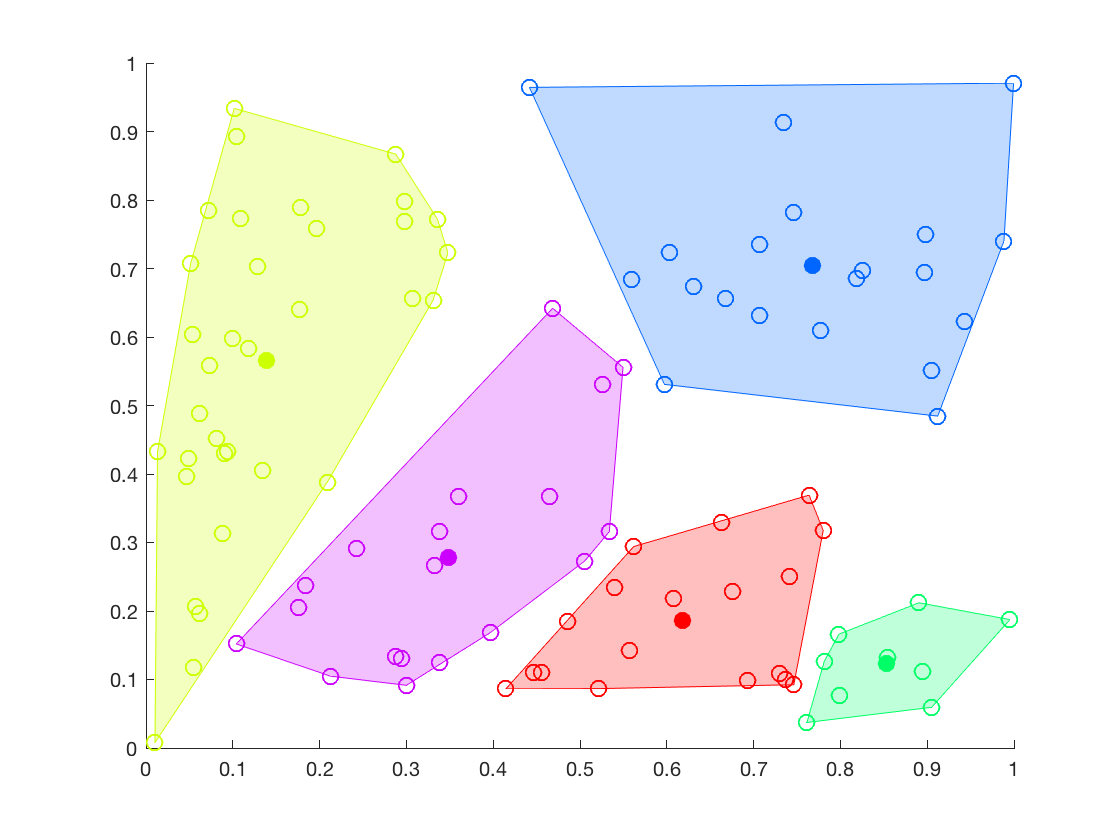
\includegraphics[width=\textwidth]{k-means_3}
    \end{subfigure}
    \begin{subfigure}[b]{0.25\textwidth}
        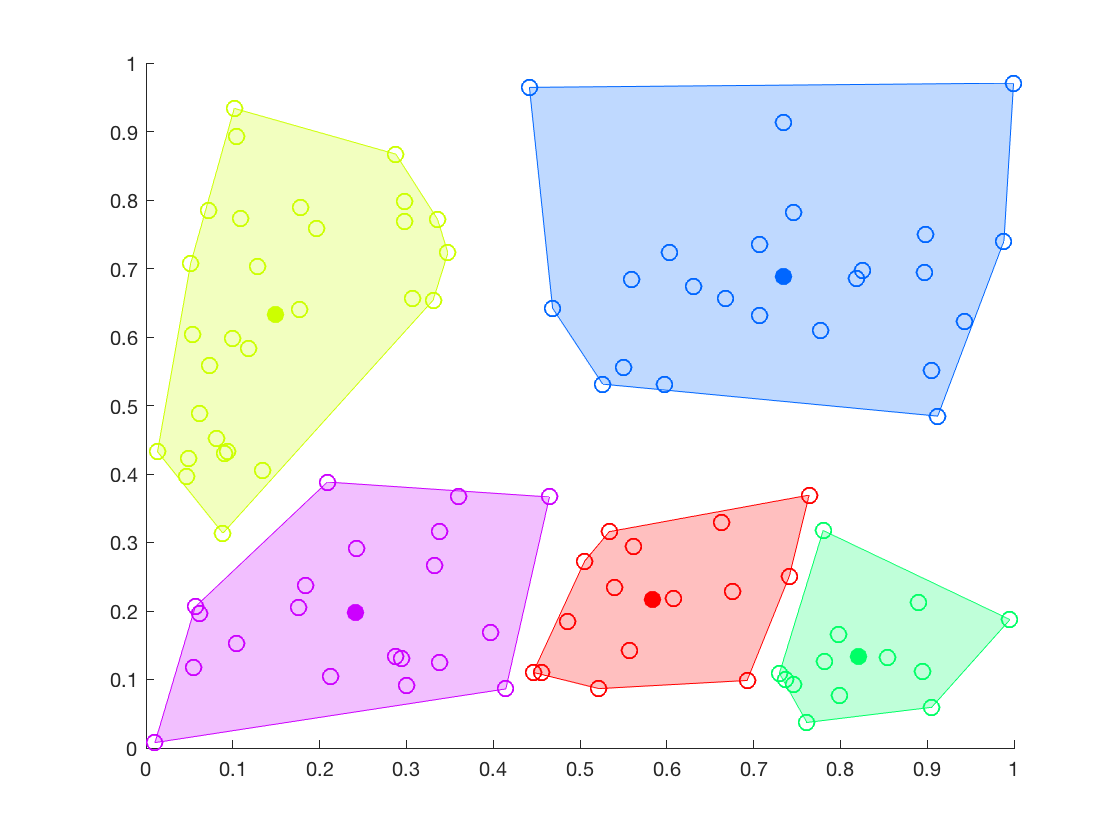
\includegraphics[width=\textwidth]{k-means_4}
    \end{subfigure}
    \begin{subfigure}[b]{0.25\textwidth}
        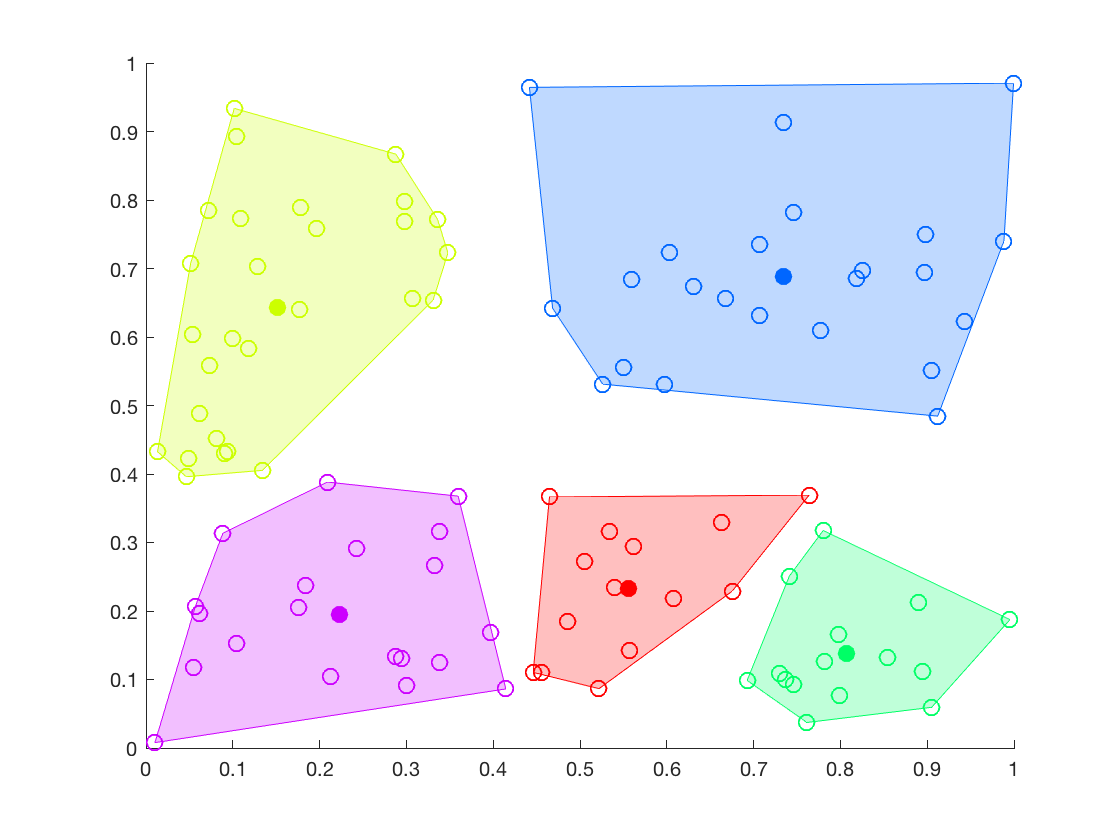
\includegraphics[width=\textwidth]{k-means_5}
    \end{subfigure}
    \begin{subfigure}[b]{0.25\textwidth}
        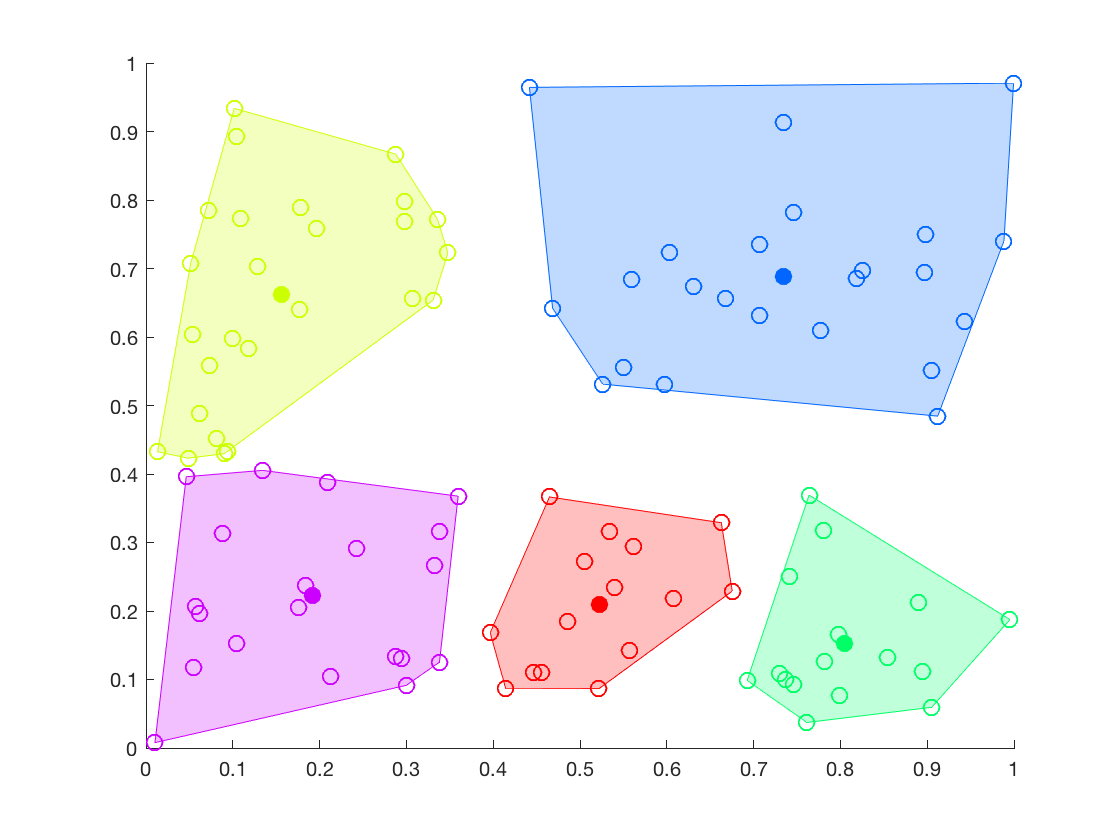
\includegraphics[width=\textwidth]{k-means_6}
    \end{subfigure}
    \begin{subfigure}[b]{0.25\textwidth}
        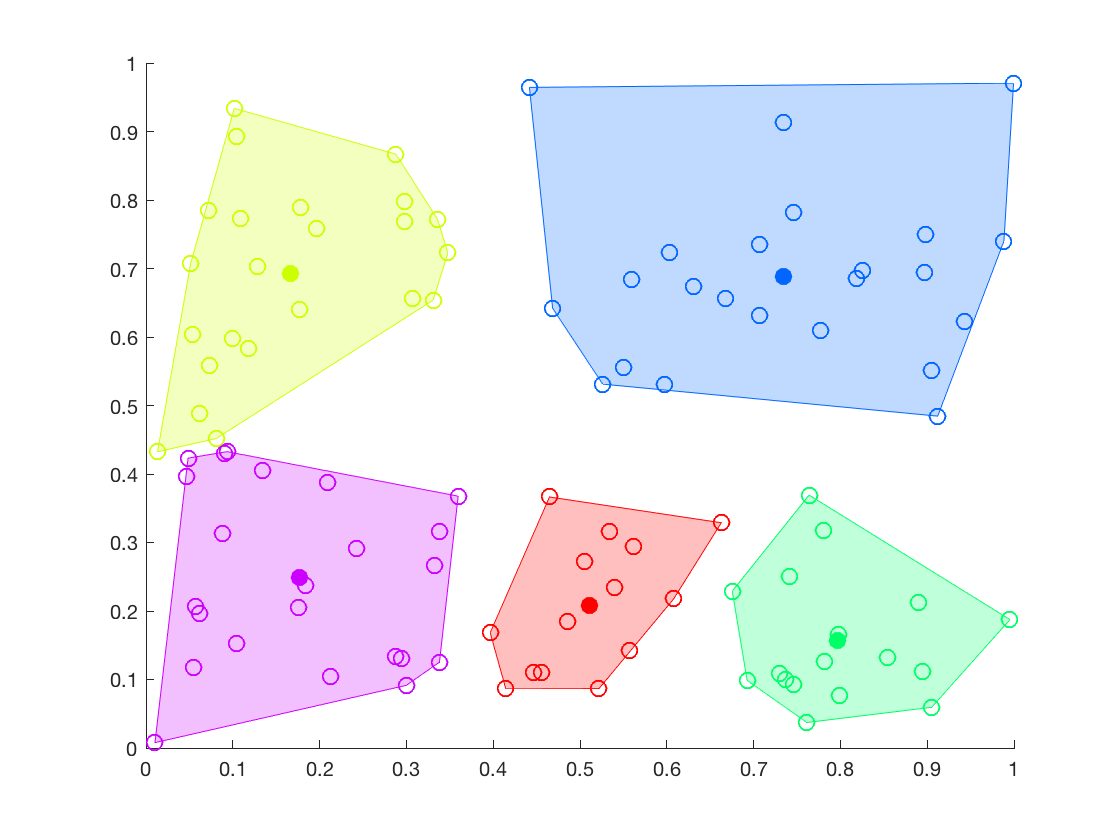
\includegraphics[width=\textwidth]{k-means_7}
    \end{subfigure}
    \begin{subfigure}[b]{0.25\textwidth}
        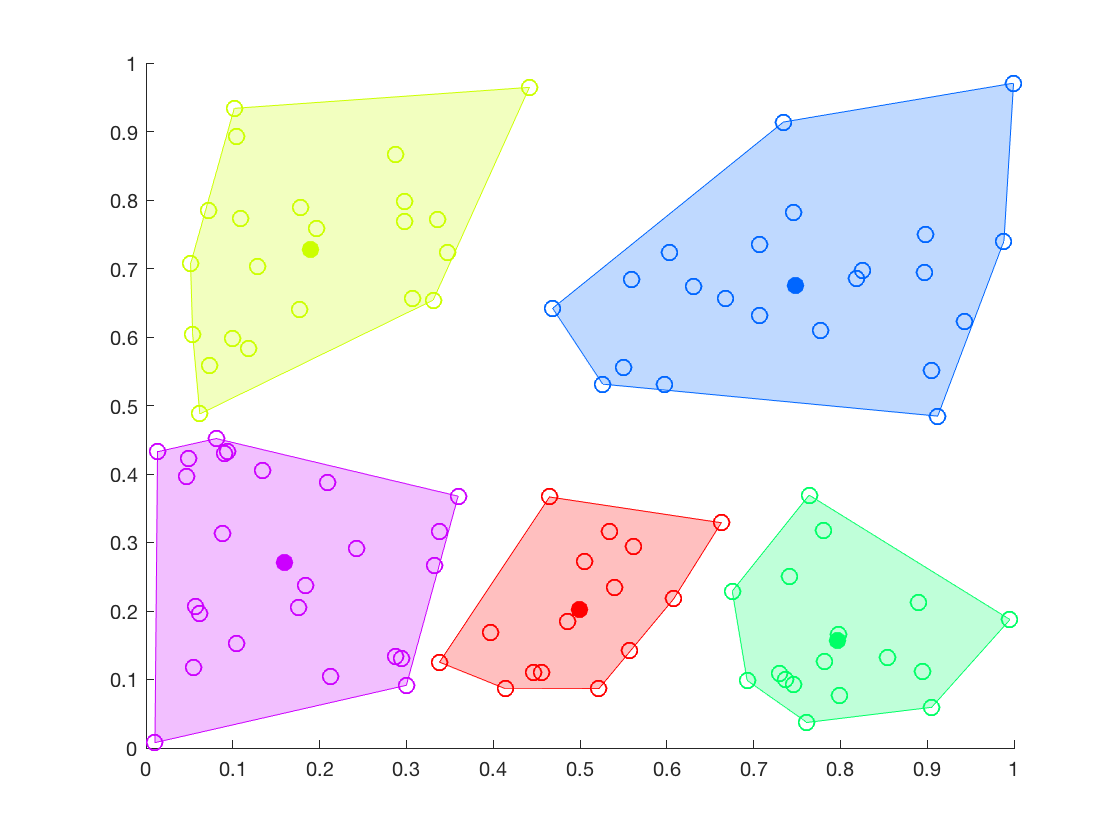
\includegraphics[width=\textwidth]{k-means_8}
    \end{subfigure}
    \begin{subfigure}[b]{0.25\textwidth}
        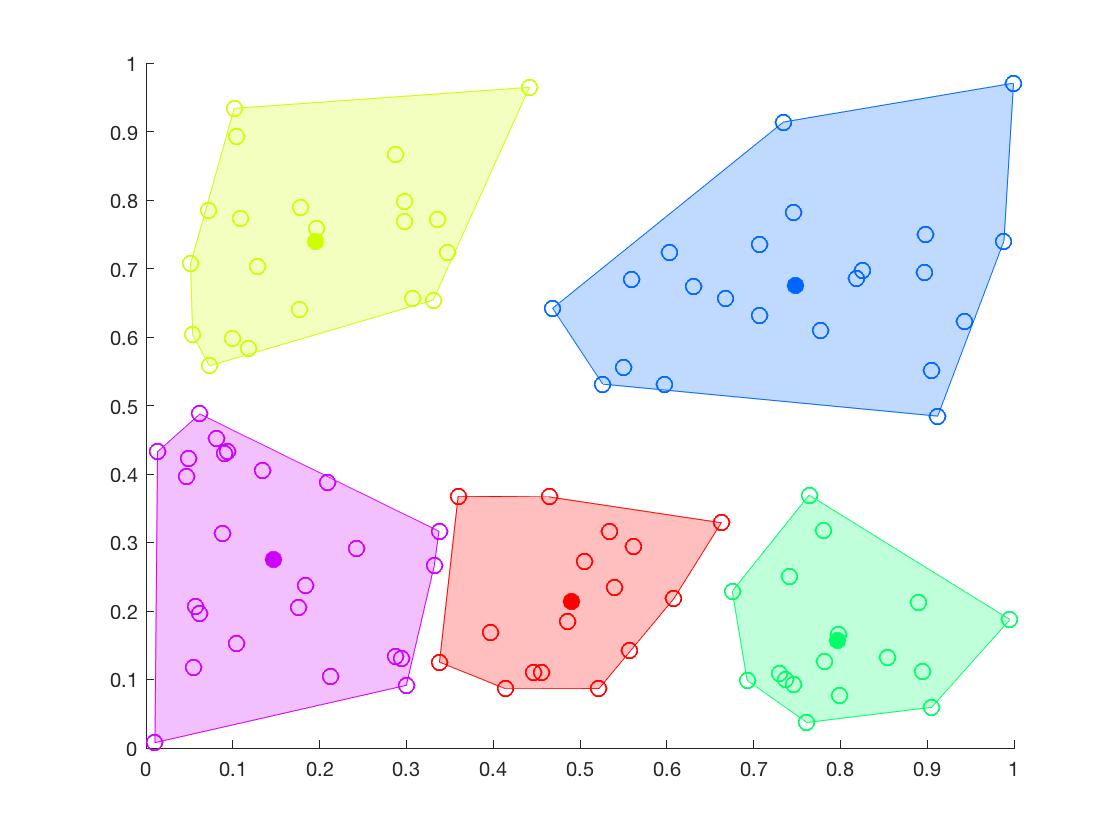
\includegraphics[width=\textwidth]{k-means_9}
    \end{subfigure}
    \begin{subfigure}[b]{0.25\textwidth}
        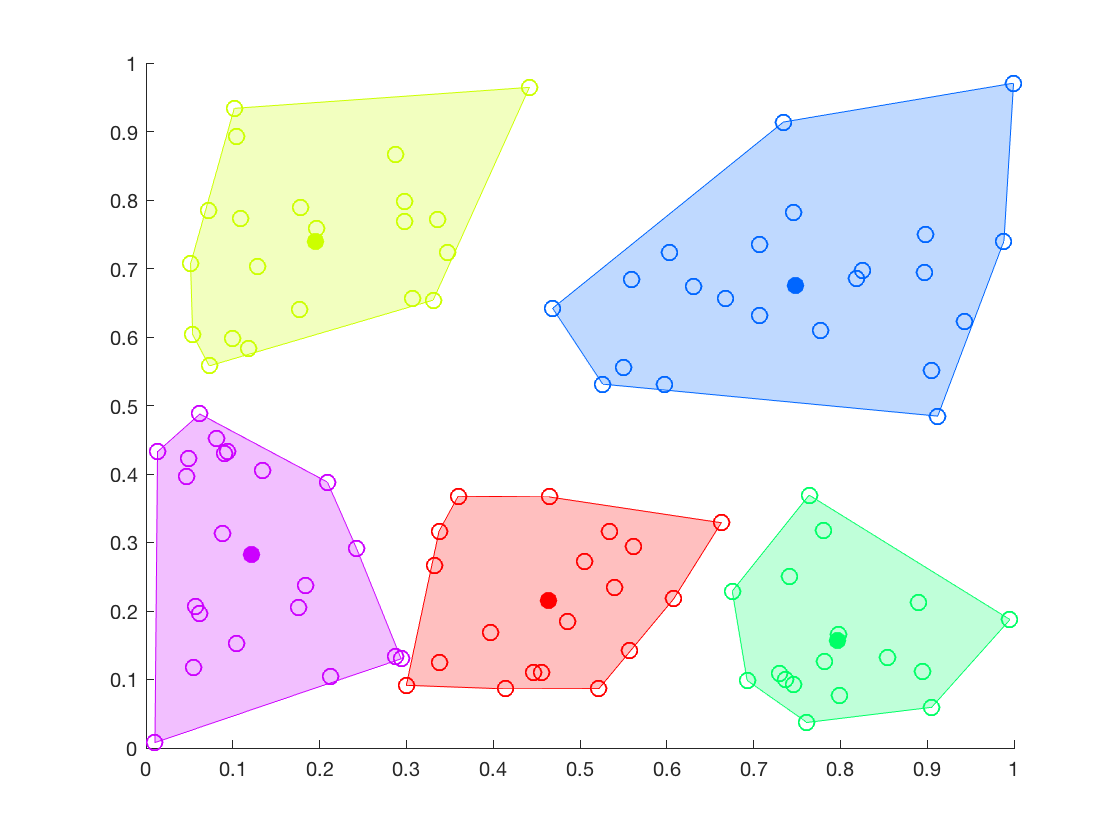
\includegraphics[width=\textwidth]{k-means_10}
    \end{subfigure}
    \begin{subfigure}[b]{0.25\textwidth}
        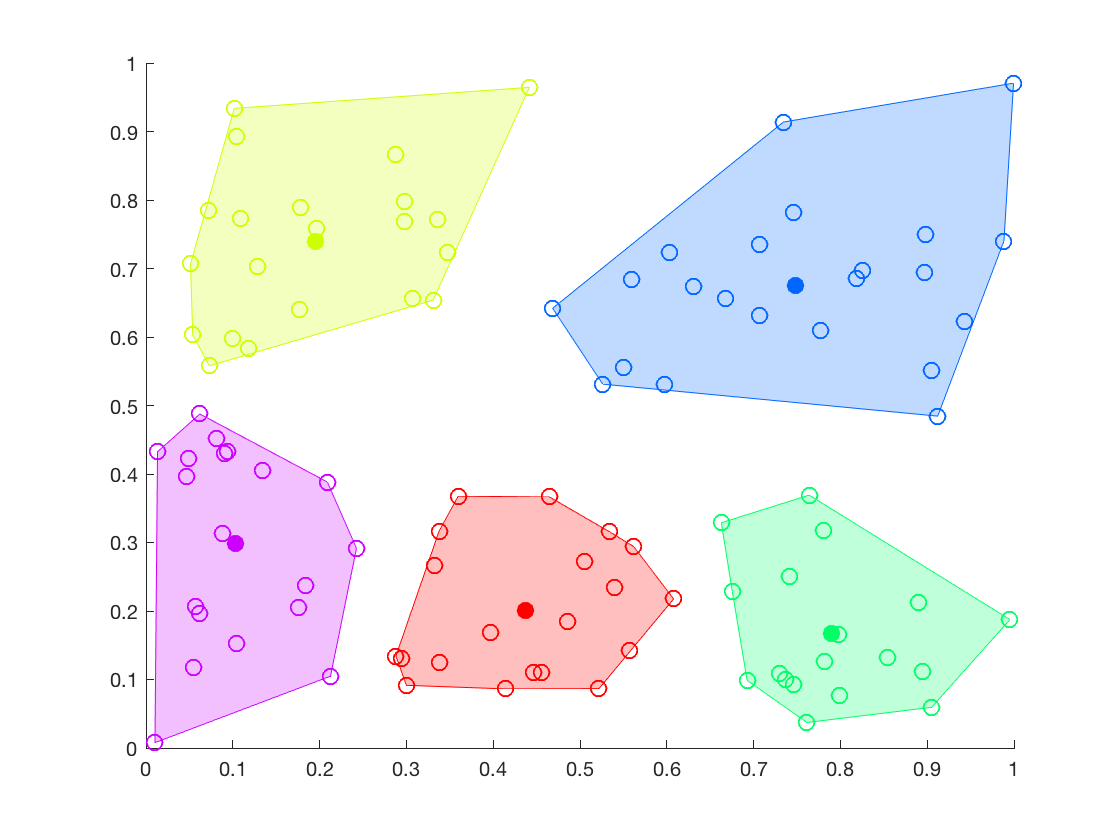
\includegraphics[width=\textwidth]{k-means_11}
    \end{subfigure}
    \caption{Series of K-Means Iterations}\label{fig:K-Means}
\end{figure}

\subsection{Hierarchical Agglomerative Clustering Algorithm}
The hierarchical agglomerative clustering algorithm is also conceptually simple:
\begin{itemize}
	\item assign each point to its own cluster
	\item compute the distance between all pairs of clusters, merge the pair of clusters that are closest to each other
  	\item recomputing the centroids of all clusters and the distances between all pairs of centroids
  	\item repeat steps until the number of clusters meets our requirement
\end{itemize}

\begin{figure}[t!]
    \centering
    \begin{subfigure}[b]{0.3\textwidth}
        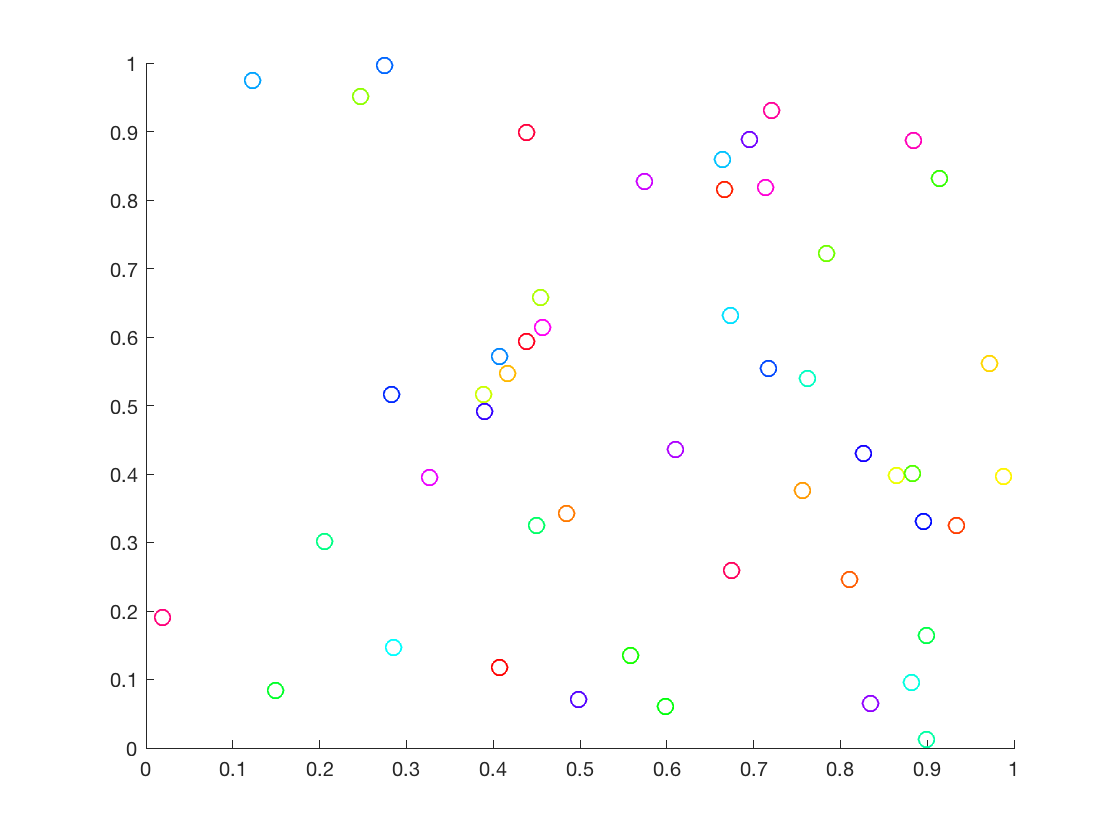
\includegraphics[width=\textwidth]{ha_1}
    \end{subfigure}
    \begin{subfigure}[b]{0.3\textwidth}
        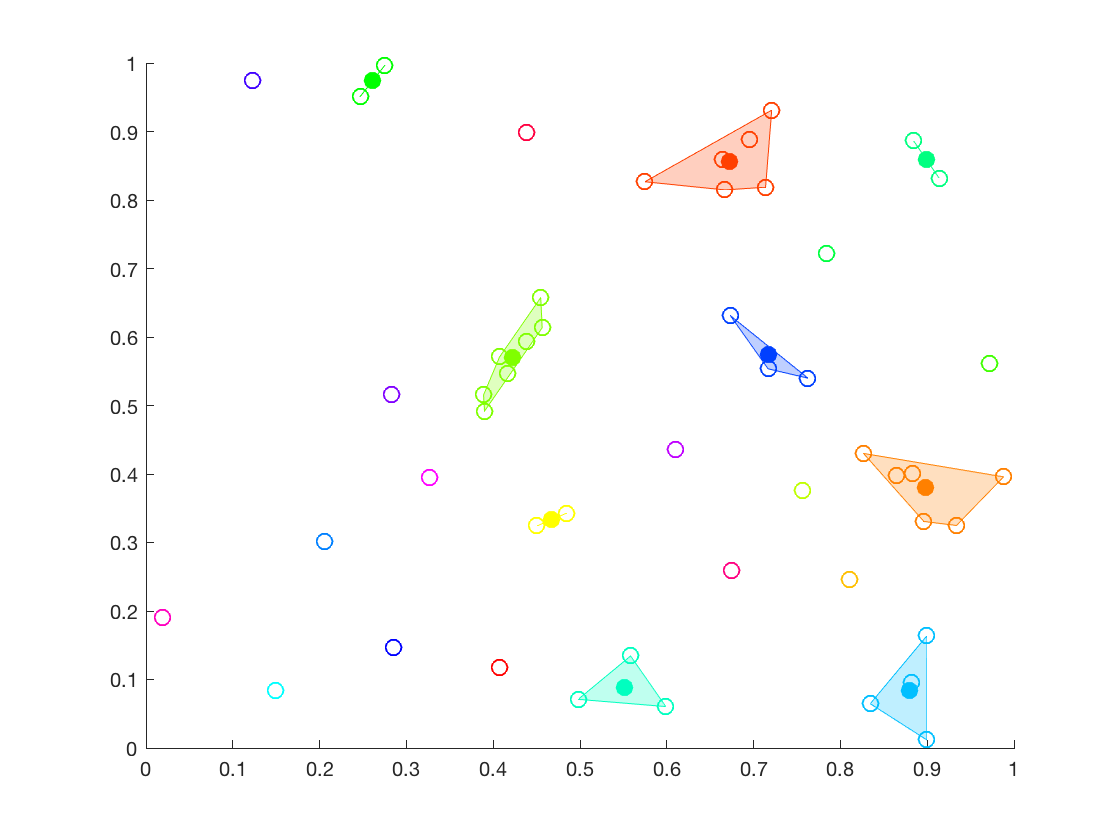
\includegraphics[width=\textwidth]{ha_2}
    \end{subfigure}
    \begin{subfigure}[b]{0.3\textwidth}
        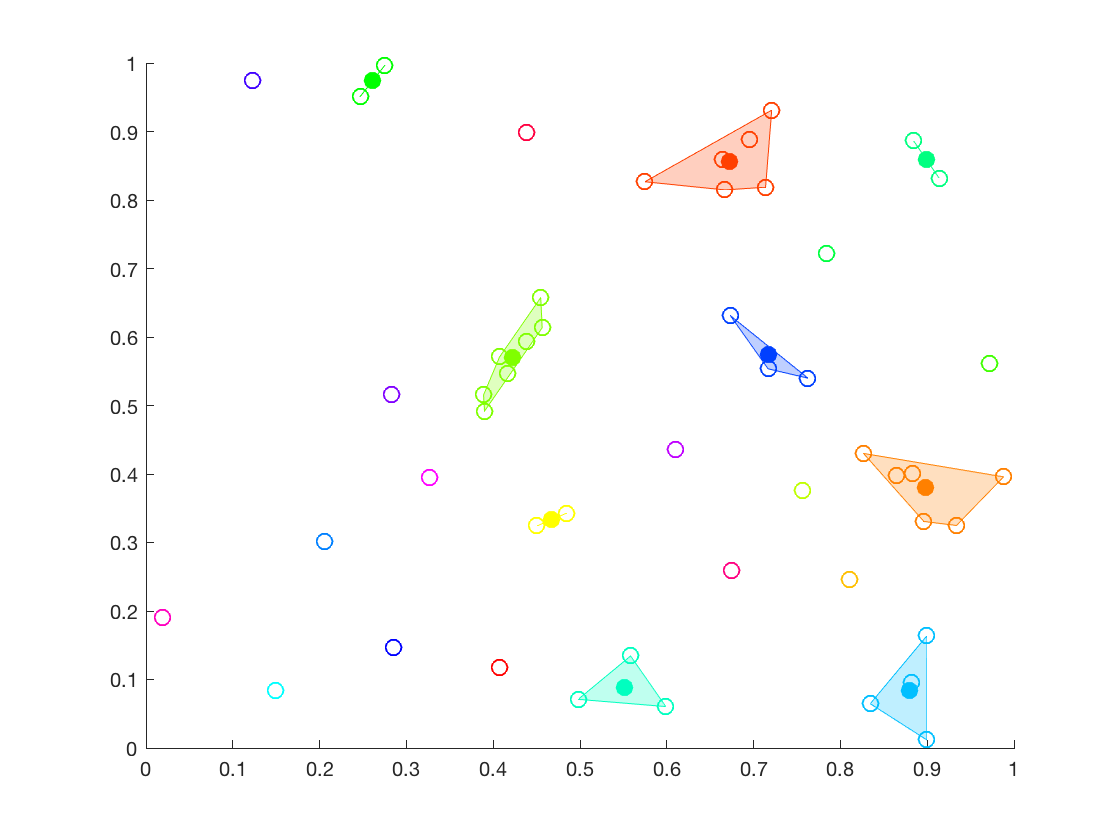
\includegraphics[width=\textwidth]{ha_3}
    \end{subfigure}
    \begin{subfigure}[b]{0.3\textwidth}
        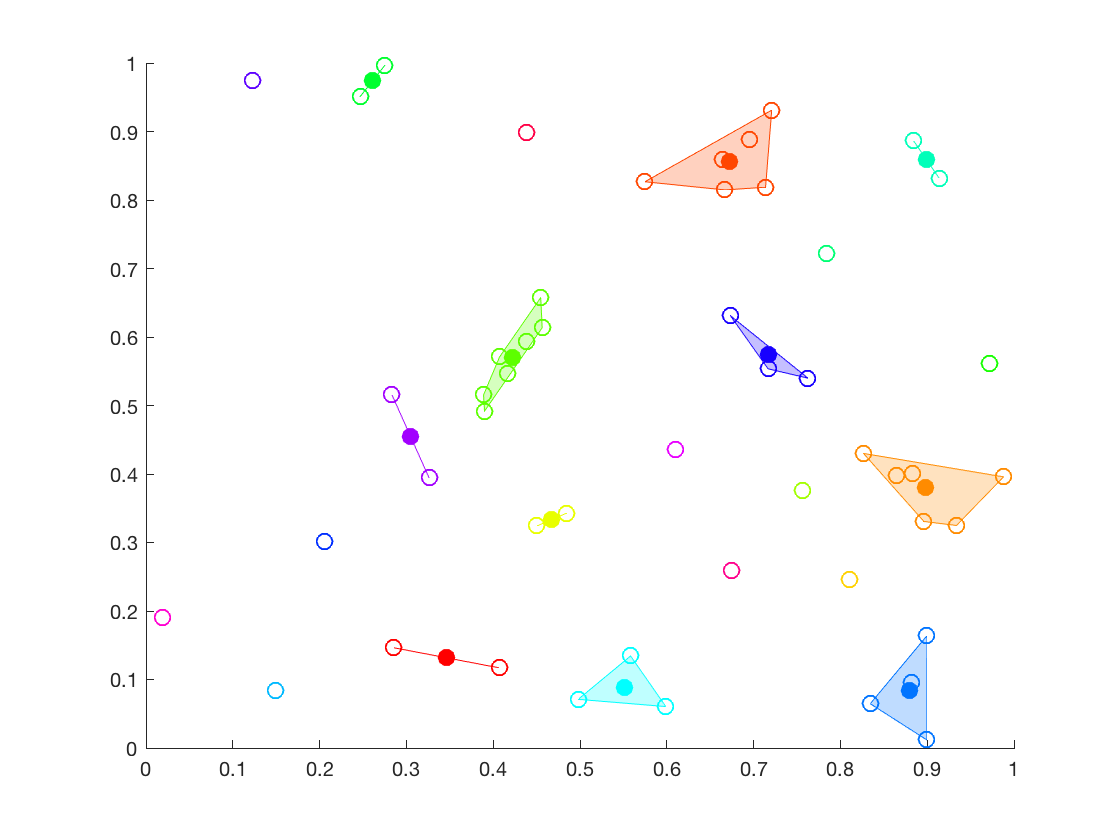
\includegraphics[width=\textwidth]{ha_4}
    \end{subfigure}
    \begin{subfigure}[b]{0.3\textwidth}
        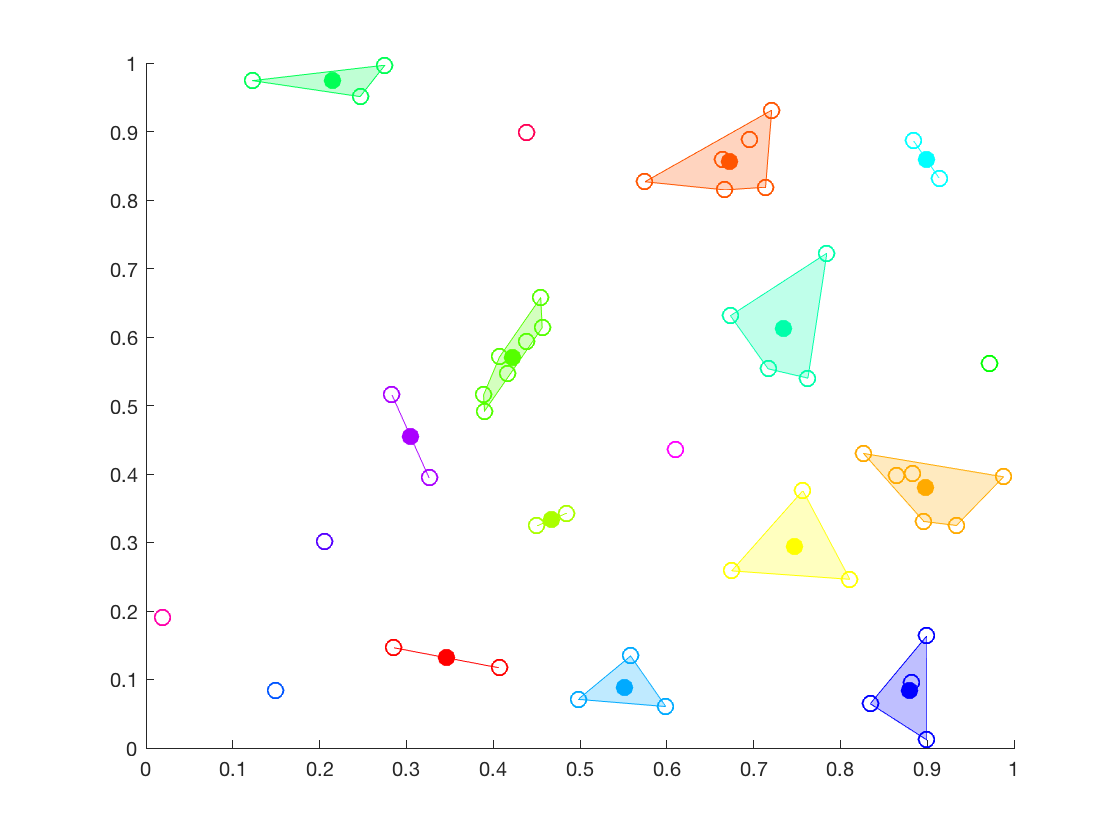
\includegraphics[width=\textwidth]{ha_5}
    \end{subfigure}
    \begin{subfigure}[b]{0.3\textwidth}
        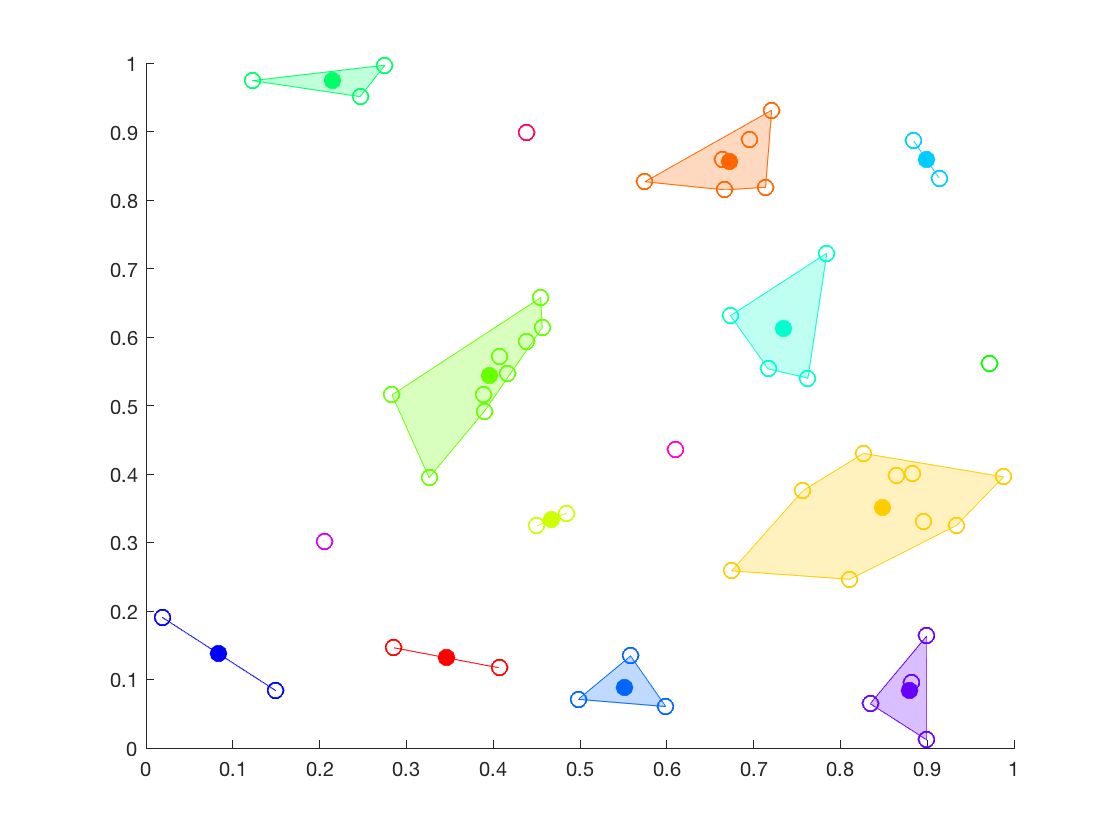
\includegraphics[width=\textwidth]{ha_6}
    \end{subfigure}
    \begin{subfigure}[b]{0.3\textwidth}
        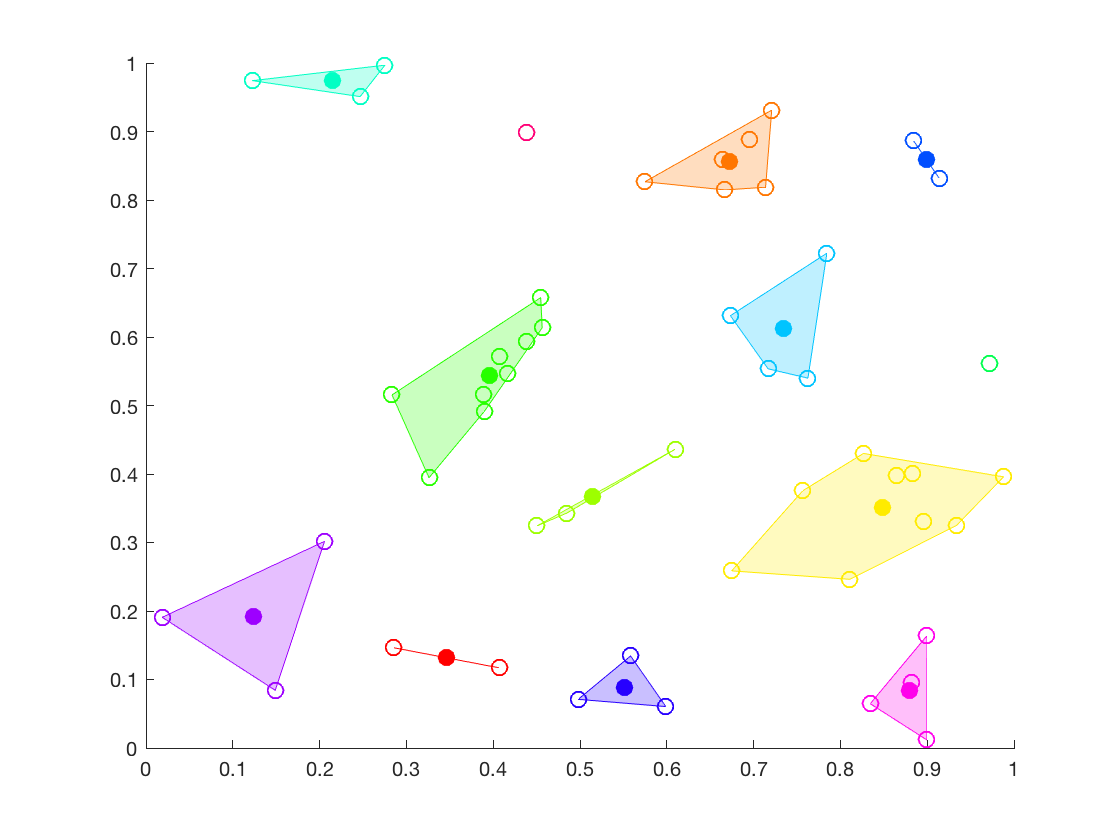
\includegraphics[width=\textwidth]{ha_7}
    \end{subfigure}
    \begin{subfigure}[b]{0.3\textwidth}
        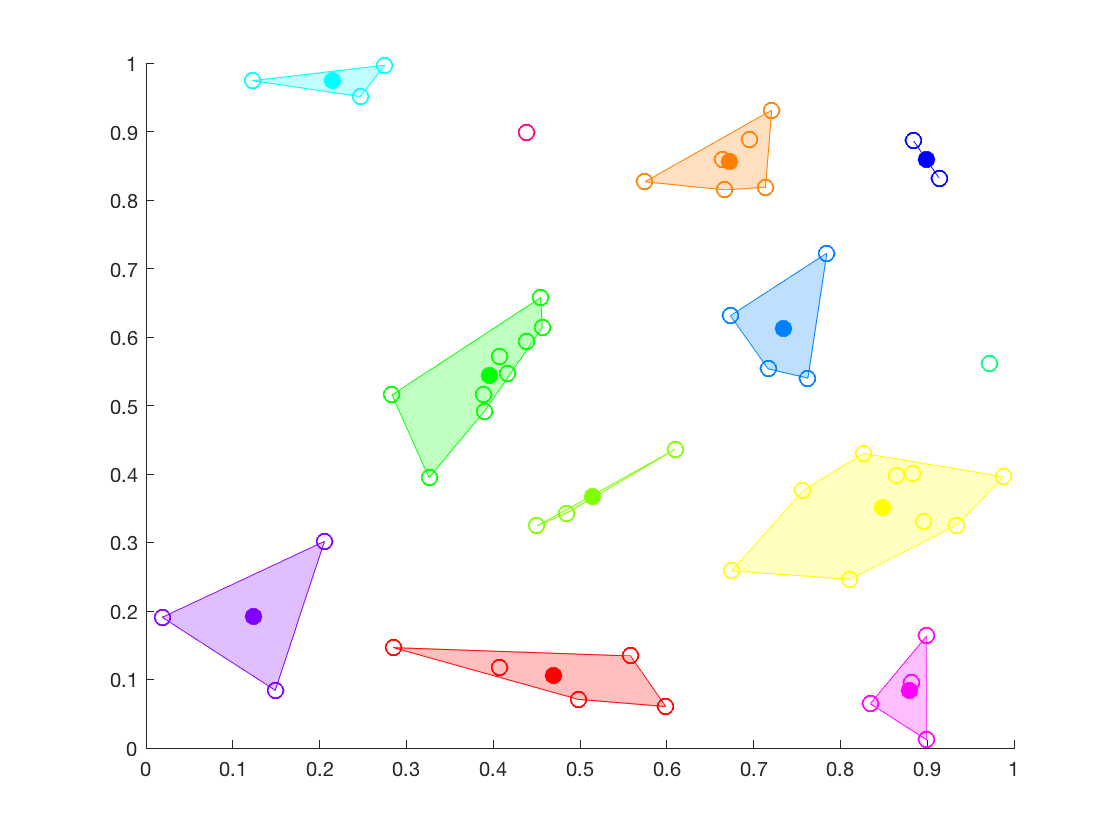
\includegraphics[width=\textwidth]{ha_8}
    \end{subfigure}
    \begin{subfigure}[b]{0.3\textwidth}
        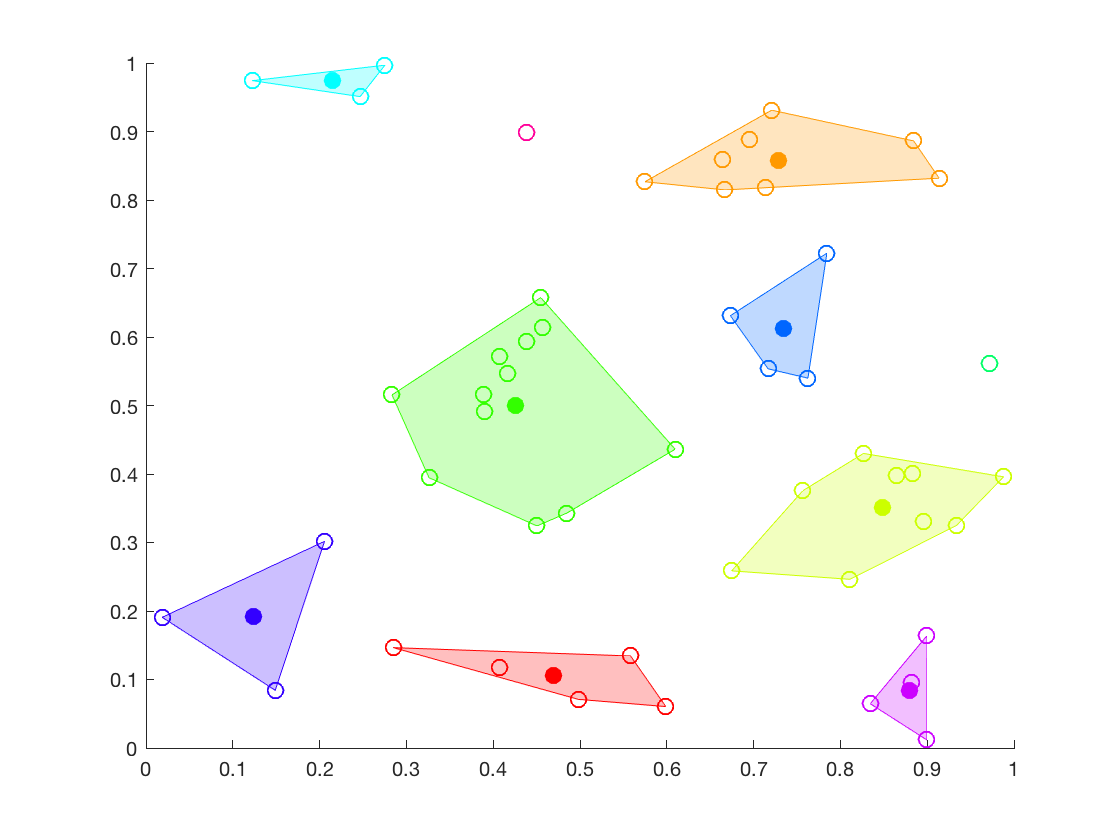
\includegraphics[width=\textwidth]{ha_9}
    \end{subfigure}
    \begin{subfigure}[b]{0.3\textwidth}
        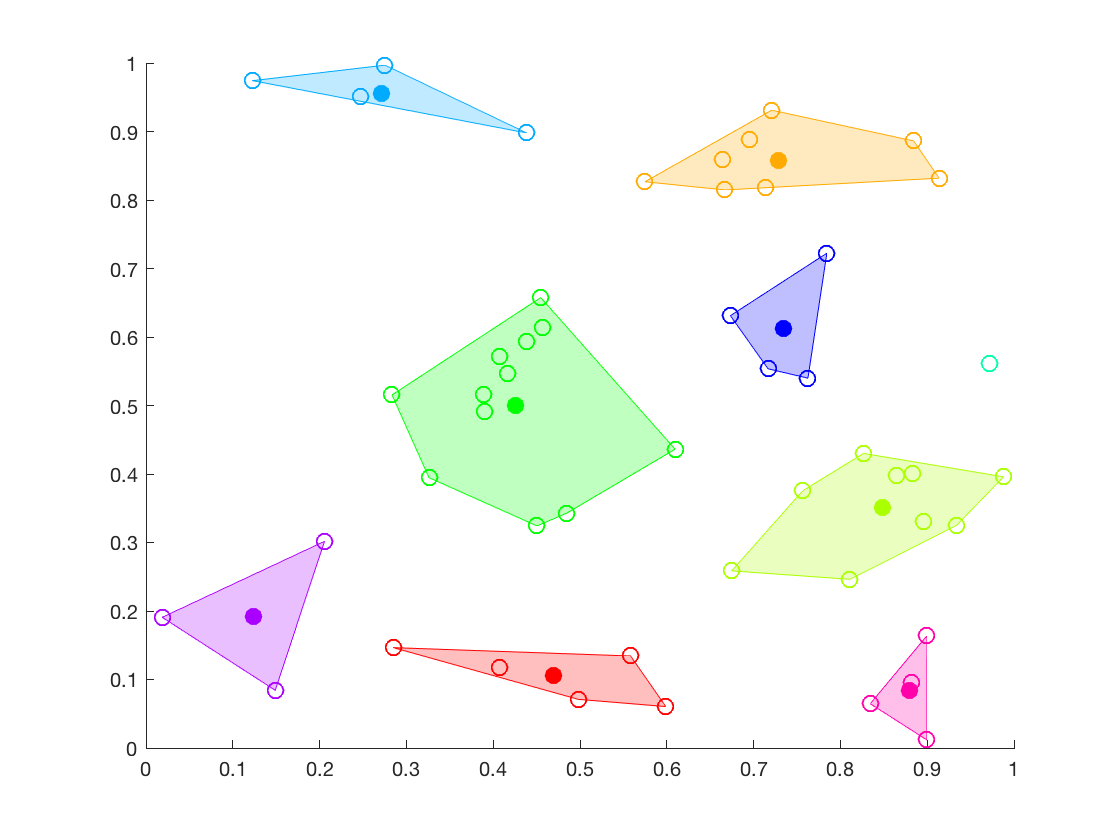
\includegraphics[width=\textwidth]{ha_10}
    \end{subfigure}
    \begin{subfigure}[b]{0.3\textwidth}
        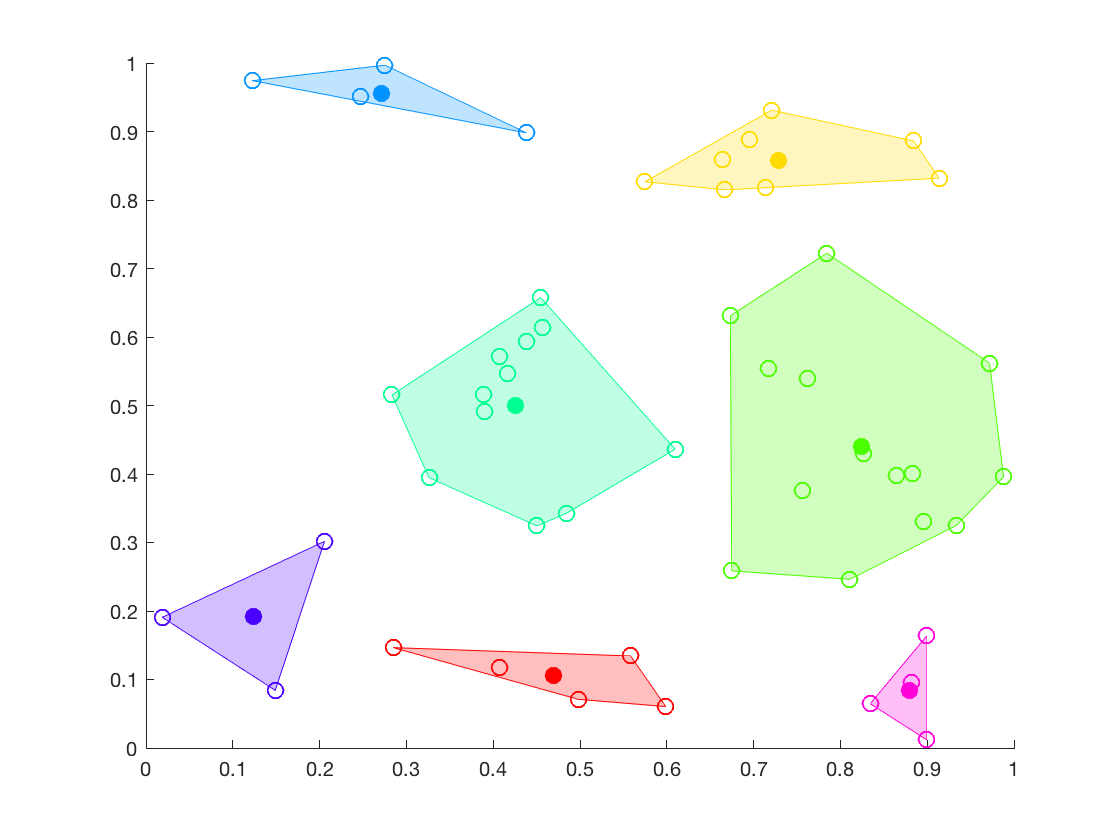
\includegraphics[width=\textwidth]{ha_11}
    \end{subfigure}
    \begin{subfigure}[b]{0.3\textwidth}
        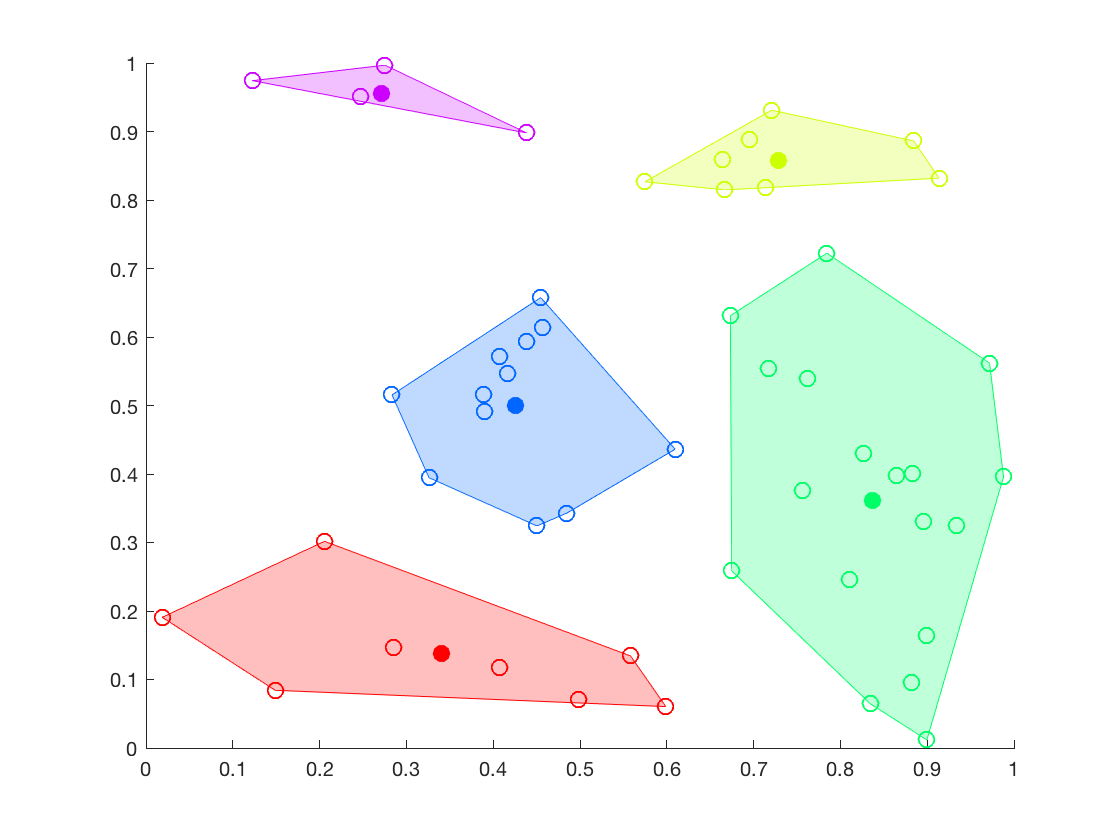
\includegraphics[width=\textwidth]{ha_12}
    \end{subfigure}
    \caption{Series of HAC Iterations}\label{fig:HAC}
\end{figure}

\section{Pixel Feature Vectors}
We need to compute some feature vector for each pixel since we are using clustering algorithm to segment an image. The feature vector for each pixel determine the qualities of segmentation. There are numerous ways to define pixel feature vectors, one of the simplest possible feature vectors for a pixel is the vector of colors for that pixel. In addition, we have the following features can be used to help segment an image.

\begin{description}
	\item [Color Features (RGB Channels)] \hfill \\ The RGB color feature vectors are very important since it contains the primary information of the image, we expect the pixel with similar color could cluster together
	\item [Position Features (X, Y Coordinates)] \hfill \\The position feature vector is also an important information in one image, the pixel with similar position (close to each other) can be clustered together
	\item [Gradient Features (Magnitudes and Directions)] \hfill \\ The gradient feather can  be helpful to detecting the any big changes in the gray scale image.
	\item [Edge Features] \hfill \\ The edge feature is similar to gradient feature, it contains the information of where could be the location of the edges of the objects
	\item [Color Features (HSV Channels)] \hfill \\ HSV is an alternative representation of the RGB color model, it represents Hue, Saturation, and Lightness 
\end{description}


\subsection{Feature Normalization}
Sometimes we want to combine different types of features into one single feature vector. Usually the features from different source have different rang of values, uneven scaling between different feature vectors may cause clustering algorithms to behave poorly.
\noindent
One way for uneven scaling between different features is to have zeros mean and unit variance. We can use the following equations to calculate normalized feature vector, assume $f_{ij}$ is the value of $j^{th}$ feature for the $i^{th}$ pixel:
\begin{gather}
\mu _j = \frac{1}{n} \sum_{i=1}^{n}f_{ij} \\
\sigma_{j}^{2} = \frac{1}{n-1}\sum_{i=1}^{n}(f_{ij}-\mu_j)^2 \\
\tilde{f}_{ij} = \frac{f_{ij}-\mu_j}{\sigma _j}
\end{gather}
\noindent
The method to handle feature normalization is called standardization, there are several other methods, such as re-scaling, mean normalization and scaling to unit length.

\section{Image Segmentations}
Once we computed feature vector for each pixel, now we can compute a segmentation for the original image by applying a clustering algorithm to compute  feature vectors.
\noindent
The following figures shows some example of successful and unsuccessful image segmentations:

\subsection{Successful Segmentation}
\begin{figure}[h!]
	\centering
    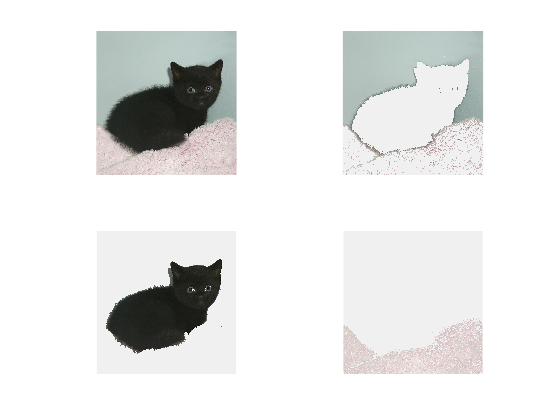
\includegraphics[scale=0.5]{seg_3_kmeans_color_true_1}
    \caption{Segmentation: K-Means, k=3, Color Feature, Normalized, Resize=1}
\end{figure}

\begin{figure}[h!]
	\centering
    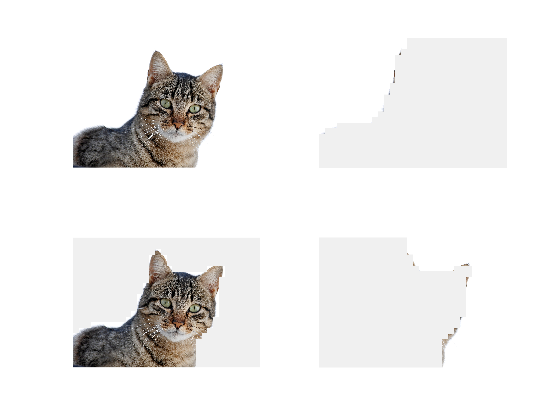
\includegraphics[scale=0.45]{seg_3_hac_color_position_true_001}
    \caption{Segmentation: HAC, k=3, Color and Position Feature, Normalized, Resize=0.01}
\end{figure}

\begin{figure}[h!]
	\centering
    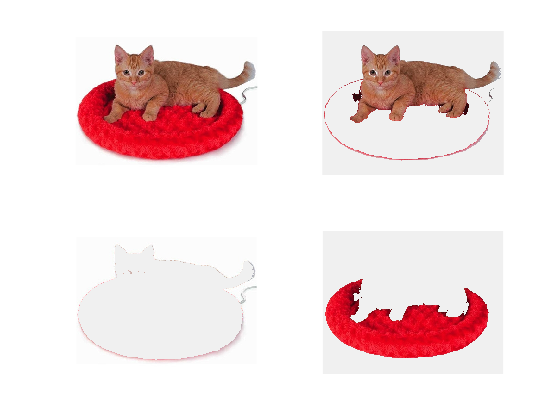
\includegraphics[scale=0.45]{seg_3_kmeans_color_false_1}
    \caption{Segmentation: K-Means, k=3, Color Feature, Un-Normalized, Resize=1}
\end{figure}

\subsection{Unsuccessful Segmentation}
\begin{figure}[h!]
	\centering
    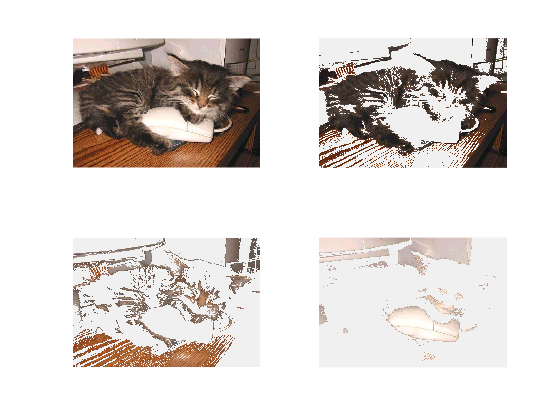
\includegraphics[scale=0.45]{seg_3_kmeans_color_true_1_us}
    \caption{Segmentation: K-Means, k=3, Color Feature, Normalized, Resize=1}
\end{figure}

\begin{figure}[h!]
	\centering
    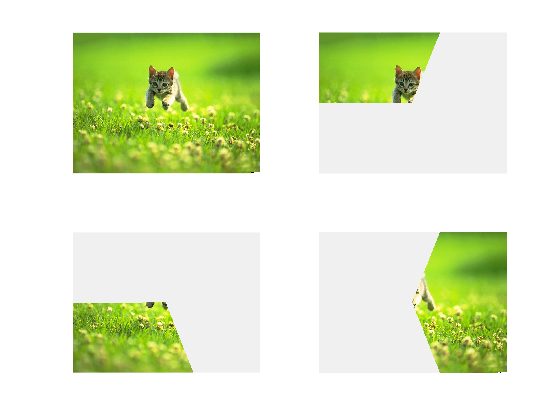
\includegraphics[scale=0.45]{seg_3_kmeans_color_position_true_1_us}
    \caption{Segmentation: K-Means, k=3, Color and Position Feature, Un-Normalized, Resize=1}
\end{figure}

\begin{figure}[h!]
	\centering
    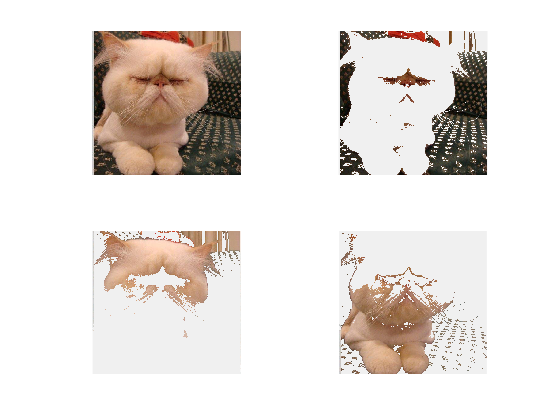
\includegraphics[scale=0.45]{seg_3_kmeans_color_position_true_1_us_2}
    \caption{Segmentation: K-Means, k=3, Color and Position Feature, Normalized, Resize=1}
\end{figure}
\vskip 10cm
\noindent
From figures as shown above, we can see for relative simple image (less objects), a small k would be sufficient. Based on the complexity of the image, different transformation would produce different quality. For more complex image, the color of the cat is not enough to identify the the object (similar color in the scene). With more than one feature transformation, normalization is important since we want each feature have the same weight. Also if we re-sized the image to small, we will not have enough pixel to separate objects.
\\
The selection of clustering algorithm affect the speed of computing significantly. K-Means is noticeable faster than HAC algorithm. However, for complicated situation, HAC outputs better results.

\section{Composite Image}
\begin{figure}[h!]
	\centering
    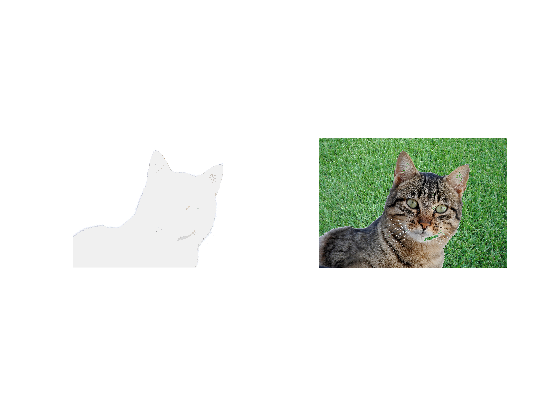
\includegraphics[scale=0.45]{grabcat1}
    \caption{Composite Grab Cat Image 1: k=3, K-Means, Position and Color Features, Normalized, Resize=0.2}
\end{figure}

\begin{figure}[h!]
	\centering
    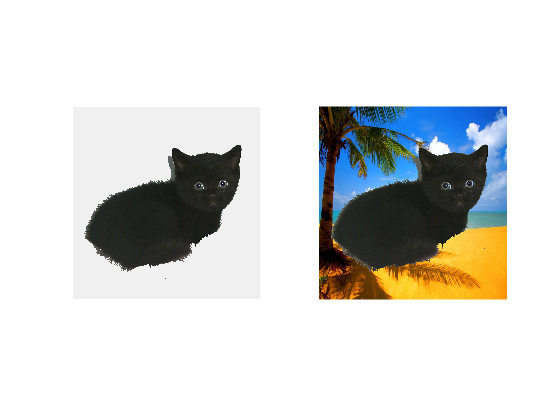
\includegraphics[scale=0.45]{grabcat2}
    \caption{Composite Grab Cat Image 2: k=3, HAC, Color Features, Normalized, Resize=0.02}
\end{figure}

\newpage
\section{Evaluation of Segmentation Parameters}
\begin{table}[h!]
\centering
\resizebox{\columnwidth}{!}{%
\begin{tabular}{l*{6}{c}r}
Feature Transform & Feature Normalization & Clustering Method & Number of Clusters & Max Pixels & Mean Accuracy \\
\hline
Color & Yes & K-Means & 10 & 10000 & 0.9150  \\
Color & Yes & K-Means & 3 & 10000 & 0.8566  \\
Color+Position & Yes & K-Means & 10 & 10000 & 0.9069  \\
Color+Gradient & Yes & K-Means & 10 & 10000 & 0.8713  \\
Color+Edge & Yes & K-Means & 10 & 10000 & 0.8924  \\
Color+HSV & Yes & K-Means & 10 & 10000 & 0.9088  \\
Color & Yes & HAC & 10 & 500 & 0.8774  \\
Position & Yes & HAC & 10 & 500 & 0.8273  \\
Color+Position & Yes & HAC & 10 & 500 & 0.8995  \\
Color+Position+Gradient & Yes & HAC & 10 & 500 & 0.8585  \\
Color+Position+Gradien+Edge & Yes & HAC & 10 & 500 & 0.8547  \\
Color+Position+Gradien+Edge+HSV & Yes & HAC & 10 & 500 & 0.8642  \\
\end{tabular}}
\end{table}

\vskip 2cm
\section{Reference}
$https://en.wikipedia.org/wiki/Feature\_scaling$

\end{document}